\documentclass[runningheads]{llncs}

\usepackage[T1]{fontenc}
\usepackage[utf8]{inputenc}
\usepackage{amsmath,amssymb}
\usepackage{graphicx}
\usepackage{booktabs}
\usepackage{float}
\usepackage{url}
\usepackage{algorithm}
\usepackage{algpseudocode}

\graphicspath{{figures/}}
\raggedbottom

\begin{document}

\title{Implementation of an Intrusion Prevention System for Mitigating DoS Attacks in Industrial Control Networks Based on PLC and Industrial Switch Protection}
\titlerunning{IPS for DoS Mitigation in ICS}

\author{Alberth Jesus Vigo Saldaña\textsuperscript{*} \and
Manuel Oswaldo Juarez Mayo \and
Jose Alfredo Valdez Reyes \and
Javier Eduardo Villegas Vidal \and
Jesús Moises Martin Villar Castillo}
\authorrunning{A. J. Vigo Saldaña et al.}

\institute{Universidad Nacional de Trujillo, Trujillo, Peru\\
\email{\{t1022700221,t1022701121,t1052702321,t1512700721,t052700420\}@unitru.edu.pe}\\
\textsuperscript{*} Corresponding author: t1022700221@unitru.edu.pe}

\maketitle

\begin{abstract}
Industrial Control Systems (ICS) are increasingly exposed to cyberattacks because operational technology is connected to IP networks, and denial-of-service (DoS) attacks threaten the availability of Programmable Logic Controllers (PLCs).
This paper presents an inline Intrusion Prevention System (IPS) architecture that protects a PLC behind a VLAN-segmented virtual industrial switch, built with free software (QEMU/KVM, Open vSwitch, nftables, Suricata, and OpenPLC), and evaluates it in a reproducible virtual testbed; the evaluation measures the availability of the PLC service, not the performance of switch hardware.
Four conditions (no attack; firewall and VLANs only; Suricata in alert mode; Suricata in drop mode) are compared under SYN, UDP, ICMP, and Modbus/TCP floods, with 10 repetitions per combination (130 runs), confidence intervals, and non-parametric tests.
The IPS in drop mode removed 99.7--100\,\% of the volumetric attack packets before the PLC network, but the legitimate SCADA client received valid replies to only 42--49\,\% of its scheduled requests, because the IPS machine became the bottleneck.
The Modbus/TCP flood stopped the PLC runtime in most runs, and a rate-based rule produced false positives on the legitimate client.
Code and raw data are available online.
\keywords{Industrial Control Systems \and Intrusion Prevention System \and DoS Mitigation \and PLC Protection \and SCADA Networks \and Cybersecurity}
\end{abstract}

\section{Introduction}\label{sec:introduction}
Industrial Control Systems (ICS) are the technological foundation of critical infrastructures such as energy, manufacturing, transportation, and water treatment. The integration of Operational Technology (OT) with Information Technology (IT) and Industrial IoT improved connectivity and efficiency, but it also exposed industrial networks, devices, and supervisory systems to cyber threats. Modern ICS rely on Ethernet and TCP/IP industrial protocols that facilitate interoperability and remote access and introduce new vulnerabilities \cite{Gillen2020ICS,Tama2022IDS}.

Denial-of-Service (DoS) attacks are among the most critical threats, because they disrupt the availability of industrial services by overwhelming devices or networks with malicious traffic. The interruption of the communication between Programmable Logic Controllers (PLCs) \cite{Raman2021ICS}, Human Machine Interfaces (HMIs), and SCADA systems can cause operational instability, safety risks, and economic losses. Unlike conventional IT systems, industrial networks require high availability and real-time responsiveness, which makes them particularly vulnerable to flooding \cite{Benka2025ICS}. PLCs are among the most critical components because they interact directly with the physical process, yet many were designed for reliability rather than security, with limited authentication and encryption \cite{Yu2019IDS}, and protocols such as Modbus/TCP, Profinet, and EtherNet/IP were developed without integrated security \cite{Yu2019IDS}.

Intrusion Prevention Systems (IPS) combine traffic inspection, signature-based detection, anomaly analysis, and automated response to block malicious activity before it reaches industrial operations \cite{Tama2022IDS,Varghese2022DigitalTwinIDS}. However, many studies focus on theoretical analyses, machine-learning models, or intrusion detection without implementing an inline prevention architecture \cite{Makrakis2021ICS,Bhamare2020ICS}, and few measure experimentally what an inline IPS does to PLC availability under DoS attacks.

The objective of this research is to design, implement, and experimentally evaluate an inline Intrusion Prevention System (IPS) that protects the availability of a PLC placed behind a VLAN-segmented virtual industrial network under four flooding attacks. The evaluation is built around a controlled comparison of four conditions (no attack, firewall and VLAN segmentation only, Suricata in alert mode, and Suricata in drop mode) so that the effect of the IPS can be separated from that of the firewall and the segmentation.

The main contributions of this work are:
\begin{itemize}
    \item A reproducible testbed built only with free software (QEMU/KVM, Open vSwitch, nftables, Suricata, OpenPLC) and a scripted run protocol, with the code and the raw measurements publicly available (see Data and Code Availability).
    \item An experimental comparison of the four conditions under SYN, UDP, ICMP, and Modbus/TCP floods, with 10 repetitions per combination (130 runs), 95\,\% confidence intervals, and non-parametric tests.
    \item Metric definitions that separate legitimate from malicious traffic, and a second, independent source (traffic mirrors and packet-count conservation) for every claim about attack traffic removed by the IPS.
    \item Findings that limit the benefit of inline prevention in this testbed: the IPS becomes the bottleneck under volumetric floods, the Modbus/TCP flood crashes the PLC runtime in most runs, and a threshold-based rule produces false positives on the legitimate SCADA client.
\end{itemize}

The paper is organized as follows: Section~\ref{sec:background} gives the background and related work, Section~\ref{sec:method} the method and metrics, Section~\ref{sec:case-study} the architecture and the experimental setup, Section~\ref{sec:results} the results, and Section~\ref{sec:conclusions} the conclusions; the data and code availability closes the paper.

\section{Background}\label{sec:background}
\subsection{Industrial Control Systems and PLCs}
Modern ICS architectures include Supervisory Control and Data Acquisition (SCADA) systems, Distributed Control Systems (DCS), Programmable Logic Controllers (PLCs), Remote Terminal Units (RTUs), Human Machine Interfaces (HMIs), and industrial networks that often keep legacy protocols designed without security mechanisms \cite{Zhu2011Taxonomy}. Their integration with Ethernet and Internet-based technologies improved interoperability but increased cybersecurity exposure \cite{Bhamare2020ICS,Kayan2021ICPS}. Industry 4.0 and IIoT paradigms connect industrial devices through standard TCP/IP protocols and cloud services \cite{Souza2021SmartManufacturing}, which expands the attack surface to malware, unauthorized access, and denial-of-service attacks \cite{Pedreira2021Industry40}.

PLCs automate electromechanical processes in real time: they read sensor inputs, run the control logic, and drive actuators in manufacturing, energy, and process control \cite{Makrakis2021ICS}. Many PLCs were designed for isolated environments and present weak authentication, insecure firmware updates, unencrypted communications, and insufficient traffic filtering, which exposes the process to command injection, unauthorized access, and denial of service \cite{Nicholson2021ICSAttacks}.

\subsection{Denial-of-Service (DoS) Attacks}
Common DoS techniques in industrial networks are SYN, ICMP, and UDP floods and protocol-specific floods against Modbus/TCP. They fall into bandwidth exhaustion, resource exhaustion, or protocol vulnerability exploitation \cite{Specht2004DDoS}, and may exhaust CPU, saturate links, or overload buffers. Incident reports describe flooding of the communication stack of widely used PLCs that causes restarts or loss of process control \cite{Chabrow2016ICS}. The effect of a flood can be summarized as $R_{attack} > R_{processing}$: the traffic generation rate exceeds the processing capacity of the device or of the network element that has to forward it.

\subsection{Intrusion Prevention Systems (IPS)}
Unlike intrusion detection systems, an IPS works inline in the communication path and can inspect, filter, and mitigate in real time \cite{Raman2021ICS}. Industrial IPS solutions combine signature-based detection, anomaly-based detection, behavioral analysis, and protocol-aware inspection \cite{Yu2019IDS}, which are the standard classification of detection methods \cite{Scarfone2007IDS}. Signature-based approaches match known patterns with rules; anomaly-based approaches use statistical or learning models, and keeping false positives low usually requires reference models of the industrial protocol \cite{Liao2013IDS}.

Industrial protocols such as Modbus/TCP, EtherNet/IP, Profinet, DNP3, and OPC UA carry the exchange between PLCs, SCADA, sensors, and actuators \cite{Pan2020PLC}. Modbus/TCP is widely used for its simplicity but has no authentication, encryption, or integrity checks, so it is exposed to interception, replay, command injection, and denial of service \cite{Yu2019IDS}. Industrial security strategies therefore combine IPS, firewalls, and VLAN segmentation \cite{Lin2021Protocols}.

\subsection{Inline Prevention with Suricata and NFQUEUE}
An IPS can be deployed inline on a Linux router by diverting forwarded packets from the kernel packet filter to a user-space engine. In this work the \texttt{nftables} \texttt{queue} statement sends the forwarded packets to \texttt{NFQUEUE}, and Suricata returns a verdict for each packet: \emph{accept}, or \emph{drop} when a rule with the \texttt{drop} action matches. With the \texttt{alert} action Suricata only logs the match and accepts the packet, so any packet that does not reach its destination in that mode was lost for another reason, such as an overflowing queue. An inline IPS therefore adds an element to the data path whose capacity bounds the traffic the network can forward \cite{fraunholz2018industrial}.

\subsection{Related Work and Positioning}
Surveys of intrusion detection in industrial control systems \cite{Liao2013IDS,Bhamare2020ICS,ahmed2019survey} describe signature-based, anomaly-based, and protocol-aware techniques, and most experimental studies evaluate detection models, often based on machine learning \cite{Tama2022IDS,Raman2021ICS}. Fraunholz et al.\ propose and implement a concept for reactive protection of industrial networks with an IPS \cite{fraunholz2018industrial}, and Yu et al.\ propose a two-stage intrusion detection system for Ethernet/IP networks \cite{Yu2019IDS}. In contrast with detection-centred studies, this work measures what an inline, rule-based IPS does to the availability of a PLC service, using a reproducible free-software testbed, a baseline that isolates the firewall and the segmentation, repeated runs with statistical analysis, and independent sources for the traffic that the IPS removes.

\section{Research Method}\label{sec:method}
This research adopted an applied and experimental methodology aimed at evaluating the effectiveness of an Intrusion Prevention System (IPS) for mitigating Denial-of-Service (DoS) attacks in industrial control networks. The methodological framework was designed to simulate realistic industrial communication scenarios involving Programmable Logic Controllers (PLCs), industrial switches, SCADA components, and malicious traffic generation within a controlled virtual environment.

The experimental process consisted of designing an industrial network architecture, implementing an IPS-based protection mechanism, generating multiple DoS attack scenarios, capturing network traffic, and analyzing performance indicators related to availability, packet loss, latency, and attack mitigation efficiency. The methodology allowed comparative analysis between industrial environments operating with and without IPS protection under identical attack conditions.

Recent industrial cybersecurity studies emphasize the importance of experimental validation in ICS security research due to the operational complexity and real-time communication requirements of industrial infrastructures. Additionally, experimental approaches facilitate the evaluation of industrial cybersecurity mechanisms under controlled attack scenarios while preserving reproducibility and performance analysis capabilities.

\subsection{Research Approach}
The research followed an applied, quantitative, and experimental approach focused on evaluating cybersecurity mechanisms in industrial communication environments. The applied research methodology was selected because the study aims to solve a practical industrial cybersecurity problem associated with the protection of PLC-based communication infrastructures against denial-of-service attacks.

\begin{table}[htbp]
\caption{Operationalization of Research Variables} 
\scriptsize 
\begin{tabular}{l c c c} 
\toprule
\textbf{Indicator} & \textbf{Index} & \textbf{\begin{tabular}{@{}c@{}}Unit of\\Measurement\end{tabular}} & \textbf{Unit of Observation} \\
\midrule
Packet Loss & [0--100] & \% & Network Traffic \\
Network Latency & [0--1000] & ms & PLC/SCADA Comm. \\
PLC Availability & [0--100] & \% & Industrial Services \\
Detection Rate & [0--100] & \% & IPS Detection \\
CPU Utilization & [0--100] & \% & IPS Devices \\
Throughput & [0--1000] & Mbps & Network Performance \\
\bottomrule
\end{tabular}
\end{table}

A quantitative approach was adopted to measure the operational impact of cyberattacks and evaluate the effectiveness of the proposed IPS architecture using measurable network performance indicators such as packet loss, response latency, attack detection rate, throughput, and device availability. Quantitative methodologies are widely employed in industrial cybersecurity research due to their ability to provide objective performance evaluation and statistical analysis of network behavior under attack conditions.

The experimental component of the research consisted of implementing a virtual industrial network environment where multiple attack scenarios were executed under controlled conditions. The study employed comparative analysis between a control environment without IPS protection and an experimental environment incorporating IPS-based traffic filtering and attack mitigation mechanisms. This experimental methodology enabled direct evaluation of the operational improvements introduced by the IPS deployment.

\subsection{Experimental Design}
The experimental design will follow a quasi-experimental approach based on comparative evaluation between two industrial network scenarios:

\begin{enumerate}
    \item Control Group (CG): Industrial network operating without IPS protection.
    \item Experimental Group (EG): Industrial network operating with IPS protection enabled.
\end{enumerate}

Both environments maintained identical industrial communication architectures, including PLC devices, industrial switches, SCADA components, and industrial communication protocols. The primary difference between the two scenarios was the implementation of inline IPS protection in the experimental environment.

The experimental infrastructure will simulate an industrial communication network composed of:

\begin{itemize}
    \item OpenPLC controllers
    \item SCADA communication services
    \item industrial Ethernet switching
    \item segmented industrial traffic
    \item and attack-generation nodes.
\end{itemize}

Different denial-of-service attack scenarios will be executed from an attacker node using Kali Linux tools to generate malicious traffic targeting industrial communication devices and PLC infrastructure. The attacks included:

\begin{itemize}
    \item SYN Flood attacks
    \item ICMP Flood attacks
    \item UDP Flood attacks
    \item and Modbus TCP flooding attacks.
\end{itemize}

\begin{table}[htbp]
\caption{Experimental Attack Scenarios}
\label{tab:attacks}
\centering
\scriptsize
\begin{tabular}{l c c c}
\toprule
\textbf{Attack Type} & \textbf{Duration} & \textbf{Protocol} &
\textbf{Target} \\
\midrule
SYN Flood & 5 min & TCP & PLC Services \\
ICMP Flood & 5 min & ICMP & Network Nodes \\
UDP Flood & 5 min & UDP & SCADA Services \\
Modbus Flood & 5 min & Modbus/TCP & PLC Devices \\
\bottomrule
\end{tabular}
\end{table}

The experimental process consisted of the following phases:

Baseline traffic generation under normal industrial communication conditions.
Execution of denial-of-service attacks without IPS protection.
Activation and configuration of IPS security policies.
Re-execution of attack scenarios with IPS protection enabled.
Traffic capture and performance analysis using monitoring tools.
Comparative evaluation of operational metrics.

This methodology enabled analysis of the operational behavior of industrial communication infrastructures before and after IPS deployment while maintaining controlled and reproducible testing conditions.

\subsection{Variables}
The research considered one independent variable and multiple dependent variables associated with industrial network performance and cybersecurity effectiveness.

\subsubsection{Independent Variable}
\textbf{IPS Implementation}

The independent variable corresponds to the deployment and activation of the Intrusion Prevention System (IPS) within the industrial communications infrastructure. The IPS will be configured to perform online packet inspection, malicious traffic filtering, industrial protocol inspection, and attack mitigation during denial-of-service attack scenarios.

\subsubsection{Dependent Variables}
\textbf{Packet Loss}
Packet loss represents the percentage of industrial communication packets that failed to reach their destination during network transmission. High packet loss may affect industrial process synchronization and operational continuity.

\textbf{Network Latency}
Network latency refers to the communication delay between industrial devices such as PLCs, SCADA servers, and industrial switches. Increased latency may negatively affect deterministic industrial communications and real-time operations.

\textbf{PLC Availability}
PLC availability measures the operational continuity of industrial controllers during attack conditions. Availability represents the percentage of operational uptime maintained during experimental execution.

\textbf{Attack Detection Rate}
The detection rate evaluates the effectiveness of the IPS in identifying and mitigating malicious traffic generated during denial-of-service attacks.

\textbf{CPU Utilization}
CPU utilization measures the computational load experienced by industrial devices and IPS components during traffic flooding scenarios.

\textbf{Throughput}
Throughput represents the amount of industrial communication traffic successfully processed by the network infrastructure during normal and attack conditions.

Recent studies indicate that these variables are widely employed for evaluating industrial cybersecurity mechanisms and traffic protection architectures in ICS environments.

\subsection{Metrics}
To evaluate the effectiveness of the proposed IPS architecture, several quantitative metrics will be used during the experimental process.

\subsubsection{Packet Loss Rate}
The packet loss rate measures the percentage of packets lost during communication transmission.

\begin{equation*}
\text{Packet Loss} = \frac{Packets_{\text{sent}} - Packets_{\text{received}}}{Packets_{\text{sent}}} \times 100
\end{equation*}

\noindent\textbf{Where:}
\begin{itemize}
    \item $Packets_{\text{sent}}$ represents the total transmitted packets.
    \item $Packets_{\text{received}}$ represents the successfully received packets.
\end{itemize}

\subsubsection{Detection Rate}
The detection rate evaluates the capability of the IPS to identify malicious traffic generated during attack scenarios.

\[
\text{Detection Rate} = \frac{\text{Detected Attacks}}{\text{Total Attacks}} \times 100
\]

\noindent\textbf{Where:}
\begin{itemize}
    \item $\text{Detected Attacks}$ represents the number of successfully identified attacks.
    \item $\text{Total Attacks}$ represents the total executed attacks.
\end{itemize}

\subsubsection{Availability}
Availability measures the operational continuity of industrial devices during attack conditions.

\[
\text{Availability} = \frac{\text{Uptime}}{\text{Total Time}} \times 100
\]

\noindent\textbf{Where:}
\begin{itemize}
    \item $\text{Uptime}$ represents the total operational time.
    \item $\text{Total Time}$ represents the total experimental duration.
\end{itemize}

\subsubsection{Network Latency}
Network latency was measured using packet round-trip time (RTT) analysis between industrial devices and PLC communication nodes.

\[
\text{Latency} = \text{Receive Time} - \text{Send Time}
\]

\subsubsection{Throughput}

Throughput evaluates the amount of successfully transmitted industrial traffic per unit of time.

\[
\text{Throughput} = \frac{\text{Total Data Transferred}}{\text{Transmission Time}} \times 100
\]

\subsection{Tools}
The experimental environment was implemented using virtualization, industrial simulation, network analysis, and cybersecurity tools capable of reproducing realistic industrial communication scenarios.

\subsubsection{OpenPLC}
OpenPLC was employed as the industrial controller platform for simulating PLC communications and industrial process control. OpenPLC provides support for industrial automation protocols and programmable control logic within virtualized environments.

\subsubsection{Kali Linux}
Kali Linux was utilized as the attacker environment for generating denial-of-service attacks and malicious network traffic. Kali Linux provides penetration testing tools capable of simulating SYN Flood, UDP Flood, ICMP Flood, and protocol-specific attacks.

\subsubsection{Suricata}
Suricata was implemented as the primary Intrusion Prevention System responsible for inline traffic inspection, attack detection, protocol analysis, and malicious packet filtering.

\subsubsection{Snort}
Snort was employed for comparative rule-based intrusion detection and traffic analysis within industrial communication environments.

\subsubsection{Wireshark}
Wireshark was used to capture and analyze industrial network traffic during baseline and attack conditions. Packet analysis enabled measurement of latency, packet loss, protocol behavior, and malicious traffic characteristics.

\subsubsection{GNS3}
GNS3 was utilized to simulate the industrial network topology, industrial switches, VLAN segmentation, and communication routing between industrial devices.

\subsubsection{VirtualBox}
VirtualBox was employed to host the virtual machines composing the industrial laboratory environment, including attacker systems, PLC nodes, SCADA services, and IPS infrastructure.

\section{Case Study}\label{sec:case-study}
The proposed architecture is mainly based on the approaches presented by \cite{fraunholz2018industrial} and complemented with industrial intrusion detection models proposed in \cite{sayegh2019ids}.

The architecture follows a hierarchical industrial network design based on IT/OT segmentation and the deployment of an Intrusion Prevention System (IPS) to mitigate Denial of Service (DoS) attacks targeting Programmable Logic Controllers (PLCs) and industrial switches.

The proposed solution incorporates:
\begin{itemize}
    \item Network segmentation using VLANs,
    \item Separation between IT and OT environments,
    \item Inline IPS inspection,
    \item Monitoring of industrial protocols,
    \item Protection of PLC communication channels.
\end{itemize}

According to Fraunholz et al. \cite{fraunholz2018industrial}, industrial IPS architectures should provide reactive protection mechanisms capable of identifying malicious traffic patterns and preventing attacks before they impact industrial devices.

Additionally, Ahmed et al. \cite{ahmed2019survey}, recommend the implementation of Purdue-based segmentation models to isolate operational technology (OT) networks from corporate infrastructures.

The proposed architecture aims to:
\begin{itemize}
    \item Protect PLCs against DoS attacks,
    \item Improve industrial network availability,
    \item Detect anomalous industrial traffic,
    \item Reduce propagation of attacks within OT environments,
    \item Maintain stable communication between SCADA systems and PLCs.
\end{itemize}

\subsection{Network Architecture}
The network architecture follows a layered industrial control system (ICS) design inspired by the Purdue Enterprise Reference Architecture and the IPS deployment proposed by Fraunholz et al. \cite{fraunholz2018industrial}.

The architecture separates the corporate network from the operational network using firewalls, industrial switches, VLAN segmentation, and an inline Intrusion Prevention System (IPS).

The IPS is strategically deployed between the SCADA layer and the PLC network in order to inspect traffic in real time and mitigate potential flooding attacks targeting industrial devices.

The proposed architecture includes the following components:

\begin{table}[htbp]
\caption{Components of the Proposed Industrial Architecture} 
\centering
\scriptsize
\resizebox{\columnwidth}{!}{%
\begin{tabular}{l c c}
\toprule
\textbf{Component} & \textbf{Function} & \textbf{Reference} \\
\midrule
PLC & Industrial process control & \cite{fraunholz2018industrial} \\
SCADA/HMI & Monitoring and supervision & \cite{fraunholz2018industrial} \\
Industrial Switch & VLAN segmentation and traffic control & \cite{sayegh2019ids} \\
Firewall & IT/OT network separation & \cite{ahmed2019survey} \\
IPS (Suricata/Snort) & Attack detection and mitigation & \cite{fraunholz2018industrial} \\
Monitoring Station & Traffic analysis and packet capture & \cite{sayegh2019ids} \\
Attacker Machine & DoS attack generation & Experimental environment \\
\bottomrule
\end{tabular}%
}
\end{table}


The industrial switch is responsible for managing VLAN segmentation and isolating traffic between the SCADA network and PLC devices. According to Sayegh et al. \cite{sayegh2019ids}, segmentation mechanisms improve the security posture of industrial Ethernet networks by reducing unnecessary broadcast traffic and limiting attack propagation.

The IPS performs Deep Packet Inspection (DPI) on industrial protocols such as Modbus/TCP and Ethernet/IP. This allows the detection of abnormal traffic patterns associated with DoS attacks.

The architecture also incorporates a Demilitarized Zone (DMZ) between the enterprise network and the industrial network to provide an additional security layer, as recommended in \cite{ahmed2019survey}.

\subsection{Topology}
The proposed topology follows a hierarchical Industrial Control System (ICS) architecture inspired by the Purdue Enterprise Reference Model and the distributed intrusion detection approach proposed by Mansfield et al. \cite{mansfield2020threeTier}.

The architecture separates the corporate network from the operational technology (OT) environment through the use of firewalls, industrial switches, and VLAN segmentation. An inline Intrusion Prevention System (IPS) is deployed between the SCADA layer and the PLC network to monitor and mitigate malicious traffic in real time.

The proposed topology is illustrated in Figure~\ref{fig:industrial_topology}.

\begin{figure}[H]
    \centering
    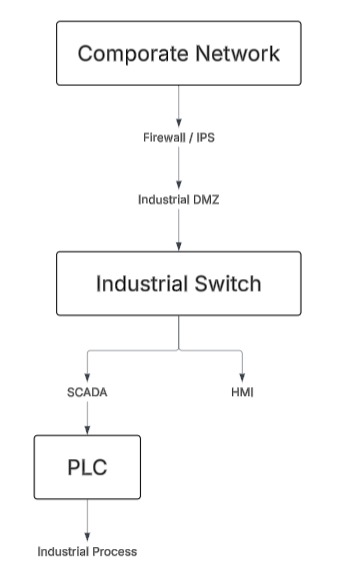
\includegraphics[width=0.3\textwidth]{network_topology.jpeg}
    \caption{Proposed industrial network topology}
    \label{fig:industrial_topology}
\end{figure}

According to Fraunholz et al. \cite{fraunholz2018industrial}, network segmentation and the implementation of a DMZ reduce the propagation of attacks within industrial environments and improve the monitoring capabilities of security systems.

The industrial switch is responsible for managing traffic isolation between VLANs and prioritizing industrial communications. Sayegh et al. \cite{sayegh2019ids}, indicate that traffic segmentation improves the resilience of industrial Ethernet networks against denial-of-service attacks.

The proposed VLAN segmentation is presented in Table~\ref{tab:vlan_segmentation}.

\begin{table}[htbp]
\caption{Proposed VLAN Segmentation} 
\scriptsize 
\begin{tabular}{l c c c} 
\toprule
\textbf{VLAN} & \textbf{Purpose} & \textbf{Reference} \\
\midrule
VLAN 10 & Corporate network & Purdue Model \\
VLAN 20 & SCADA/HMI communication & \cite{ahmed2019survey} \\
VLAN 30 & PLC network & \cite{fraunholz2018industrial} \\
VLAN 99 & Network management & Industrial segmentation practice \\
\bottomrule
\end{tabular}
\label{tab:vlan_segmentation}
\end{table}

\subsection{IPS Configuration}

The Intrusion Prevention System (IPS) configuration is based on the reactive protection architecture proposed by Fraunholz et al. \cite{fraunholz2018industrial}. The IPS is deployed in inline mode to inspect industrial traffic before it reaches PLC devices.

The IPS performs Deep Packet Inspection (DPI) on industrial communication protocols such as Modbus/TCP and Ethernet/IP. According to Sayegh et al. \cite{sayegh2019ids}, protocol-aware traffic inspection improves the detection accuracy of attacks targeting industrial control systems.

The proposed IPS configuration parameters are presented in Table~\ref{tab:ips_configuration}.

\begin{table}[htbp]
\caption{IPS Configuration Parameters} 
\centering
\scriptsize
\resizebox{\columnwidth}{!}{%
\begin{tabular}{l c c}
\toprule
\textbf{Parameter} & \textbf{Configuration} & \textbf{Reference} \\
\midrule
IPS Tool & Suricata & \cite{fraunholz2018industrial} \\
Deployment Mode & Inline & \cite{fraunholz2018industrial} \\
Protected Protocol & Modbus/TCP & \cite{sayegh2019ids} \\
Detection Method & Signature-based & \cite{fraunholz2018industrial} \\
Packet Inspection & Deep Packet Inspection (DPI) & \cite{sayegh2019ids} \\
Logging & Enabled & Security monitoring practice \\
Automatic Blocking & Enabled & Reactive protection approach \\
\bottomrule
\end{tabular}%
}
\label{tab:ips_configuration}
\end{table}


The IPS uses custom detection rules to identify traffic flooding attacks directed to the PLC communication port (TCP port 502).

An example of a Suricata detection rule is shown below:

\begin{verbatim}
alert tcp any any -> 192.168.1.10 502
(msg:"Possible Modbus TCP Flood";
flow:to_server;
threshold:type both, track by_src,
count 50, seconds 1;
sid:100001;)
\end{verbatim}

The rule detects excessive TCP requests directed to the Modbus/TCP service and generates alerts when abnormal traffic thresholds are exceeded.

According to Fraunholz et al. \cite{fraunholz2018industrial}, inline IPS deployment allows real-time mitigation actions such as:
\begin{itemize}
    \item automatic packet filtering,
    \item malicious IP blocking,
    \item rate limiting,
    \item abnormal traffic isolation.
\end{itemize}

\subsection{Attack Scenarios}

The attack scenarios were designed based on methodologies commonly used in Industrial Control System (ICS) security research to evaluate the effectiveness of intrusion prevention systems against Denial of Service (DoS) attacks.

According to Fraunholz et al. \cite{fraunholz2018industrial}, PLCs are particularly vulnerable to flooding attacks due to their limited computational resources and strict real-time communication requirements.

The experimental environment considers multiple attack scenarios targeting industrial communication services such as Modbus/TCP.

\subsubsection{Scenery 1 -- TCP SYN Flood}

The first attack scenario consists of a TCP SYN Flood directed toward the PLC Modbus/TCP service operating on port 502.

The objective of this attack is to saturate the communication resources of the PLC by generating a massive number of incomplete TCP connection requests.

The attack is generated using the \texttt{hping3} tool:

\begin{verbatim}
hping3 -S --flood -V -p 502 192.168.1.10
\end{verbatim}

According to Ahmed et al. \cite{ahmed2019survey}, SYN Flood attacks can significantly degrade the availability of industrial services and interrupt SCADA communications.

\subsubsection{Scenery 2 -- Modbus/TCP Flood}

This scenario focuses on flooding the PLC with excessive Modbus/TCP requests.

The attack simulates malicious traffic directed toward industrial communication protocols in order to overload the PLC processing capabilities.

According to Sayegh et al. \cite{sayegh2019ids}, abnormal traffic patterns in industrial Ethernet protocols can negatively affect:
\begin{itemize}
    \item PLC response time,
    \item SCADA communication stability,
    \item network throughput,
    \item industrial process availability.
\end{itemize}

The attack traffic may be generated using tools such as:
\begin{itemize}
    \item Scapy,
    \item Modbus testing utilities,
    \item custom packet generators.
\end{itemize}

\subsubsection{Scenery 3 -- ICMP Flood}

The third attack scenario consists of an ICMP Flood attack targeting the industrial network.

The objective is to consume network bandwidth and increase communication latency between SCADA systems and PLC devices.

The attack can be generated using the following command:

\begin{verbatim}
ping -f 192.168.1.10
\end{verbatim}

According to Fraunholz et al. \cite{fraunholz2018industrial}, excessive ICMP traffic may affect the stability of industrial Ethernet communications and reduce system availability.

The evaluation variables used during the experiments are presented in Table~\ref{tab:evaluation_variables}.

\begin{table}[htbp]
\caption{Evaluation Variables for Attack Scenarios} 
\centering
\scriptsize
\resizebox{\columnwidth}{!}{%
\begin{tabular}{l c c}
\toprule
\textbf{Variable} & \textbf{Description} & \textbf{Reference} \\
\midrule
Packet Loss & Lost packets during attacks & \cite{fraunholz2018industrial} \\
Latency & Communication delay & \cite{sayegh2019ids} \\
Detection Rate & IPS attack detection accuracy & \cite{mansfield2020threeTier} \\
CPU Usage & PLC resource consumption & \cite{ahmed2019survey} \\
Network Throughput & Network traffic performance & ICS performance metrics \\
Availability & Operational continuity of PLC services & \cite{fraunholz2018industrial} \\
\bottomrule
\end{tabular}%
}
\label{tab:evaluation_variables}
\end{table}


\subsection{Experimental Procedure}
The experimental procedure follows the evaluation methodologies proposed by Fraunholz et al. \cite{fraunholz2018industrial} and Mansfield et al. \cite{mansfield2020threeTier} for industrial intrusion detection and prevention systems.

The experiments are conducted in a controlled industrial network environment composed of:
\begin{itemize}
    \item PLC devices,
    \item SCADA/HMI systems,
    \item industrial switches,
    \item an inline IPS,
    \item an attacker workstation,
    \item monitoring and traffic analysis tools.
\end{itemize}

The experimental methodology is divided into five phases.

\subsubsection{Phase 1 -- Environment Setup}

The first phase consists of configuring the industrial environment and communication infrastructure.

The following components are deployed:
\begin{itemize}
    \item PLC simulation or physical PLC,
    \item SCADA monitoring software,
    \item industrial Ethernet switch,
    \item Suricata IPS,
    \item Wireshark traffic analyzer,
    \item Kali Linux attacker machine.
\end{itemize}

According to Ahmed et al. \cite{ahmed2019survey}, realistic industrial testbeds are essential for evaluating the effectiveness of security mechanisms in ICS environments.

\subsubsection{Phase 2 -- Baseline Traffic Capture}

Normal industrial communication traffic is captured before launching attacks.

The objective of this phase is to establish baseline operational behavior for:
\begin{itemize}
    \item Modbus/TCP communication,
    \item SCADA--PLC interaction,
    \item network latency,
    \item packet delivery rate.
\end{itemize}

Traffic analysis is performed using Wireshark and IPS monitoring logs.

\subsubsection{Phase 3 -- Attack Execution}

During this phase, the attack scenarios described in Section 4.4 are executed against the industrial network.

The generated attacks include:
\begin{itemize}
    \item TCP SYN Flood,
    \item ICMP Flood,
    \item Modbus/TCP Flood.
\end{itemize}

The attacks are generated from the attacker workstation connected to the OT network.

\subsubsection{Phase 4 -- IPS Activation}

The IPS is activated in inline mode with predefined detection and mitigation rules.

According to Fraunholz et al. \cite{fraunholz2018industrial}, reactive IPS mechanisms allow real-time mitigation of malicious traffic before it reaches industrial devices.

The IPS performs:
\begin{itemize}
    \item traffic inspection,
    \item malicious packet filtering,
    \item automatic alert generation,
    \item attack blocking.
\end{itemize}

\subsubsection{Phase 5 -- Performance Evaluation}

The final phase evaluates the effectiveness of the proposed architecture based on the collected metrics.

The evaluation focuses on:
\begin{itemize}
    \item IPS detection accuracy,
    \item false positive rate,
    \item reduction of malicious traffic,
    \item PLC availability,
    \item network latency,
    \item industrial communication stability.
\end{itemize}

According to Mansfield et al. \cite{mansfield2020threeTier}, performance analysis is essential to determine whether security mechanisms introduce operational overhead in industrial control environments.

\section{Results and Discussion}\label{sec:results}
All results come from 130 runs (10 per combination) measured on the platform described in Section~\ref{sec:case-study}; all values are means with 95\,\% confidence intervals unless stated otherwise. Table~\ref{tab:results} summarizes the results. The raw measurements and the scripts that produce every table and figure are in the repository of the project.

\begin{table}[H]
\caption{Results by condition and attack (mean $\pm$ 95\,\% CI, $n=10$ runs per row). Replies/issued is $A_{iss}$ and Replies/sched.\ is $A_{sch}$; Removed is the percentage of attack packets that do not reach the PLC network; PLC down is the number of runs in which the PLC runtime had stopped after the attack.}\label{tab:results}
\centering\scriptsize
\setlength{\tabcolsep}{3pt}
\begin{tabular}{llrrrrr}
\toprule
Attack & Scen. & Replies/ & Replies/ & RTT p95 & Removed & PLC\\
 & & issued (\%) & sched. (\%) & (ms) & (\%) & down\\
\midrule
None & E0 & 100.0 & 100.0 & 0.86 $\pm$ 0.01 & -- & 0/10\\
\midrule
TCP SYN & E1 & 99.2 $\pm$ 0.2 & 99.0 $\pm$ 0.3 & 260 $\pm$ 6 & 2.0 $\pm$ 0.4 & 0/10\\
 & E2 & 3.4 $\pm$ 0.9 & 0.7 $\pm$ 0.2 & 359 $\pm$ 94 & 68.8 $\pm$ 1.1 & 0/10\\
 & E3 & 75.8 $\pm$ 4.0 & 48.2 $\pm$ 9.3 & 310 $\pm$ 56 & 99.9 & 0/10\\
\midrule
UDP & E1 & 100.0 & 100.0 & 4.3 $\pm$ 0.5 & 0.0 & 0/10\\
 & E2 & 66.7 $\pm$ 16.8 & 50.4 $\pm$ 23.1 & 249 $\pm$ 109 & 54.2 $\pm$ 0.8 & 0/10\\
 & E3 & 73.3 $\pm$ 4.5 & 41.9 $\pm$ 8.2 & 346 $\pm$ 51 & 99.7 $\pm$ 0.1 & 0/10\\
\midrule
ICMP & E1 & 100.0 $\pm$ 0.1 & 100.0 $\pm$ 0.1 & 21.0 $\pm$ 1.0 & 2.2 $\pm$ 0.4 & 0/10\\
 & E2 & 49.1 $\pm$ 26.3 & 41.7 $\pm$ 27.8 & 203 $\pm$ 164 & 63.1 $\pm$ 2.1 & 0/10\\
 & E3 & 77.3 $\pm$ 5.3 & 48.7 $\pm$ 10.3 & 391 $\pm$ 22 & 100.0 & 0/10\\
\midrule
Modbus & E1 & 100.0 & 100.0 & 2.0 $\pm$ 1.3 & 0.0 & 10/10\\
 & E2 & 99.7 & 99.7 & 0.9 $\pm$ 0.8 & 0.0 & 10/10\\
 & E3 & 100.0 & 100.0 & 1.1 & 30.8 $\pm$ 3.2 & 6/10\\
\bottomrule
\end{tabular}

\end{table}

\subsection{Service Availability}
Figure~\ref{fig:avail} shows the availability of the SCADA client during the attack. The baseline E0 gives 100\,\% of valid replies and an RTT p95 of 0.86~ms. Without the IPS (E1), the SYN, UDP, and ICMP floods leave the PLC answering almost every request ($A_{iss}\geq 99.2\,\%$), although the flood reaches the PLC at 150\,000--180\,000 packets per second. With the IPS in alert mode (E2) the service degrades sharply: $A_{iss}$ is 3.4\,\% for SYN, 66.7\,\% for UDP, and 49.1\,\% for ICMP, and the runs of E2 vary a great deal (from 2.5\,\% to 83\,\% with ICMP and from 30\,\% to 85\,\% with UDP). With the IPS in drop mode (E3), $A_{iss}$ is between 73\,\% and 77\,\% for the three volumetric floods.

The closed-loop client issues fewer requests when replies are missing (for example, 119 of the 600 scheduled in E2 with SYN). Measured against the scheduled requests, the service in E3 is lower, 42--49\,\% (Fig.~\ref{fig:avail}b and Table~\ref{tab:results}). Both quantities are reported because $A_{iss}$ alone overstates the service when the PLC stops answering. The RTT p95 of the replies that do arrive (Table~\ref{tab:results}) rises from 0.86~ms (E0) to 4.3--260~ms in E1 and 200--390~ms with the IPS; in runs with very few replies it describes few observations.

\begin{figure}[H]
\centering
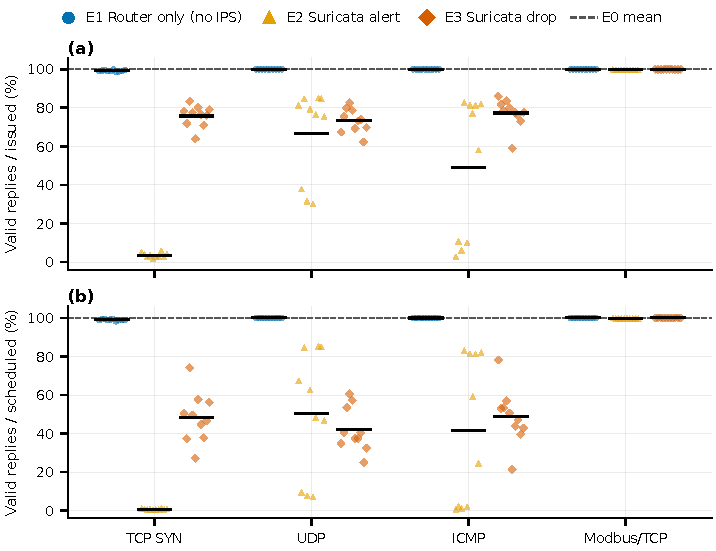
\includegraphics[width=0.88\textwidth]{r1_availability.pdf}
\caption{Availability of the SCADA client during the 60~s attack: (a) valid replies divided by requests issued; (b) valid replies divided by requests scheduled (10~Hz $\times$ 60~s). Each marker is one run, the black bar is the mean, and the dashed line is the baseline E0.}\label{fig:avail}
\end{figure}

Figure~\ref{fig:series} shows the same quantity per second. The service falls when the attack starts and recovers when it ends, except in E3, which stays at about 92\,\% in the 10~s after the attack (Section~\ref{sec:fp}). The Modbus flood does not affect the replies during the attack, but the PLC stops answering when the attack ends (Section~\ref{sec:modbus}).

\begin{figure}[H]
\centering
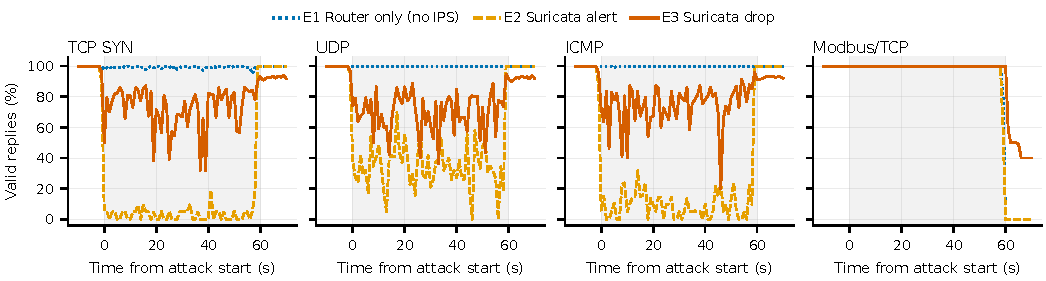
\includegraphics[width=0.92\textwidth]{r3_availability_timeseries.pdf}
\caption{Valid replies per second, averaged over the 10 runs of each combination. The shaded band is the attack window.}\label{fig:series}
\end{figure}

\subsection{Attack Traffic Removed and Resource Use}
The column Removed of Table~\ref{tab:results} gives the share of attack packets that do not reach the PLC network, measured on the mirror ports. In E3 the rules remove 99.7--100\,\% of the SYN, UDP, and ICMP floods. In E2 the rules only alert, so no packet is dropped by a rule (Suricata reported zero blocked packets), and the 54--69\,\% that disappears is due to the overflow of the \texttt{NFQUEUE}: the IPS cannot process the flood. In E1 only 0--2\,\% disappears; there is no IPS in that condition, so this difference is attributed to the packets that the capture tool discards. The packet counts are consistent across sources: for every run of E2 and E3, the packets that enter the queues (nftables counters, both directions) equal the packets dropped by the queue plus the verdicts of Suricata, with a ratio of 1.000 (0.998--1.006 in the Modbus runs of E3).

The CPU time of the virtual machines during the attack (hypervisor accounting, relative to the number of virtual CPUs) shows where the load goes. Without the IPS (E1), the PLC machine is close to saturation (82--103\,\% of its CPU) during the three volumetric floods and the Modbus flood. In E3 the PLC machine is nearly idle (about 1\,\%) because the attack does not reach it, while under the three volumetric floods the IPS machine uses all of its CPU time. The values can exceed 100\,\% because the CPU time of the hypervisor includes the emulation and I/O threads of each virtual machine. In other words, the inline IPS moves the bottleneck from the PLC to the IPS: it protects the PLC but its capacity limits the legitimate traffic that is forwarded.

\subsection{Statistical Comparison}
Table~\ref{tab:tests} gives the effect sizes and the significance of the comparisons for $A_{sch}$. Without the IPS (E1), the service is better than with the IPS (E2 and E3) in the three volumetric floods ($\delta=+1.00$, every run of E1 above every run of E2 and E3). Between E2 and E3, drop mode is better only for the SYN flood; for UDP and ICMP the difference is not significant, so the data do not show that dropping the packets by rule improves the replies over alerting them, because in both conditions the queue is the bottleneck. In the Modbus flood, E2 and E3 differ by a practically negligible amount (99.7\,\% against 100\,\%).

\begin{table}[H]
\caption{Cliff's $\delta$ for the first condition of each pair, replies/scheduled. Significance after Holm's correction: ns, not significant; $*$, $p<0.05$; $**$, $p<0.01$; $***$, $p<0.001$. Last row: $p$ values of Fisher's exact test for the PLC crashes.}\label{tab:tests}
\centering\footnotesize
\begin{tabular}{lccc}
\toprule
Attack & E1 vs E2 & E1 vs E3 & E2 vs E3\\
\midrule
TCP SYN & +1.00 (**) & +1.00 (**) & -1.00 (**)\\
UDP & +1.00 (***) & +1.00 (***) & +0.28 (ns)\\
ICMP & +1.00 (**) & +1.00 (**) & +0.00 (ns)\\
Modbus & +1.00 (***) & +0.00 (ns) & -1.00 (***)\\
\midrule
PLC down (Modbus), $p$ & 1.000 & 0.087 & 0.087\\
\bottomrule
\end{tabular}

\end{table}

\subsection{Modbus/TCP Flood and PLC Crash}\label{sec:modbus}
The Modbus flood sends valid requests at a low packet rate, so it does not degrade the replies during the attack in any condition (99.7--100\,\%). However, the OpenPLC runtime stopped when the attack ended in all runs of E1 and E2 (10 of 10) and in 6 of 10 runs of E3. In E3 the rule cuts the flow of the attacker, which sends only 46 packets per second on average, but the difference in crashes with E1 is not significant (Fisher, $p=0.087$). The Modbus flood therefore shows that the rate-based rules are not enough to protect the PLC runtime in this testbed.

\subsection{Detection and Rule Behavior}\label{sec:fp}
The rules produced alerts in all 80 runs of E2 and E3. For the SYN and ICMP floods in E3, the number of alerts is almost the number of packets processed by Suricata (99.8\,\%). For UDP, in contrast, the number of alerts is nearly constant, about 65\,500 per run, whatever the number of packets: in a calibration run with full alert logging (not part of the 130 runs), each alert corresponded to a different UDP source port, that is, one alert per flow and not one per packet. A per-packet detection rate is therefore reported only for SYN and ICMP, and the detection of UDP is reported per run and per flow.

The same calibration, repeated in four runs in drop mode with full logging, showed that the Modbus rule dropped 133--162 packets of the legitimate SCADA client per run, at the end of the 30~s attack and during the cool-down, when the client reconnects. This is a false positive of a rate-based rule, and it is consistent with the service not returning to 100\,\% right after the attack in E3 (Fig.~\ref{fig:series}). It does not explain the loss of replies during the attack, because the SCADA packets were not dropped by the rule during most of the attack. These false positives were not quantified in the 130 runs, in which the log only stored counters.

\subsection{Threats to Validity}
The measurements come from one physical host with virtual machines and a virtual switch, so absolute values (RTT, capacity of the IPS) are specific to this hardware and do not transfer to a physical PLC or industrial switch, which were not evaluated. The CPU time is measured in a virtual machine, and the capture tool discarded up to 13.8\,\% of the packets in some runs of E1. Six runs (five of E3 with ICMP and one of E1 with ICMP) started with the host colder than the others because of a defect in the temperature check of the scripts, which was corrected; their measurements are complete, and the sample does not allow attributing the lower E3 availability observed in them to the cold start. The Modbus rule was not recalibrated, and Snort was not evaluated.

\section{Conclusions and Future Research}\label{sec:conclusions}

The proposed IPS architecture effectively mitigated the impact of TCP SYN, Modbus/TCP, and ICMP flood attacks on the simulated industrial network. Experimental results showed significant reductions in packet loss and network latency, as well as improvements in PLC availability and communication performance; this demonstrates that integrating in-line Deep Packet Inspection (DPI) with network segmentation offers an effective and cost-efficient approach to protecting industrial control systems against DoS attacks.

Despite these encouraging results, certain limitations must be considered. The experimental evaluation was conducted in a virtualized environment, which cannot fully replicate the deterministic behavior or operational constraints of real-world industrial infrastructures. Furthermore, Suricata's effectiveness relies on signature-based detection rules, limiting its ability to identify unknown or zero-day attacks without prior rule updates.

Future work should focus on validating the proposed architecture in real industrial environments using commercial PLCs and industrial network equipment. Additionally, integrating hybrid detection models based on machine learning and behavioral analysis—along with evaluating additional industrial communication protocols and more sophisticated cyberattack scenarios—would enhance the applicability and robustness of the proposed solution for real-world industrial control systems.


\bibliographystyle{splncs04}
\bibliography{references}

\end{document}
